\documentclass[titlepage,12pt]{article}
\usepackage{graphicx}
\usepackage{datetime}
\usepackage{indentfirst}
\usepackage{hyperref}
\hypersetup{
colorlinks = true, % Colours links instead of ugly boxes
linkcolor = blue, % Colour of internal links
urlcolor = blue, % Colour of external links
}

\begin{document}

\tableofcontents
\newpage


\section{About LineFit}

LineFit is a simple open source program intended for academic use that allows users to fit lines to data that has both x and y error/uncertainty values. LineFit currently uses the Java 1.7 runtime and has been tested on Windows, Mac and Linux operating systems.

\subsection{History}
LineFit was started almost ten years ago as a simple command line program in C written by Don Petcher, professor of physics at Covenant College, for the Physics department at Covenant College. Since then, it has been worked on by ten students of Covenant College (a complete list can be found in the LineFit menu Help -$>$About), the most notable being Ben Hubbard who finished the basic functionalities of LineFit and Keith Rice who brought it to a completed state in the Spring of 2015. As part of finishing LineFit, the code was hosted on GitHub in order to facilitate bug fixing and feature adding. This document was created on \today ~and is current for LineFit version 0.98.3.



\subsection{Philosophy}
LineFit, in its essence, is a data graphing program designed to be used in the academic realm. The main idea that drives LineFit is just what it name implies – that data with error or uncertainty values can be fit using a line. Often times the relationship of the data is not naturally linear, but it \hyperref[sec:dataManipulation]{can be rearranged} so that the relationship becomes linear. By forcing the user to do this, it makes their life simpler in many ways because they know they are manipulating the data towards a linear fit instead of trying many complicated fits to see which matches the data best. This also forces the user to learn how to manipulate real data which is a very practical skill in the sciences.

The second driving idea behind LineFit is that fitting a line to data should be simple and intuitive. Many other graphing programs exist, but most allow many kinds of complex fits when a linear fit would often be most appropriate or, at least, work. Because of this, LineFit is designed to be straight forward and easy to understand. A major part of this is to only to allow linear fits because it will be in an intuitive and well known form for people in the sciences and this also allows for simpler menus and fewer options. In addition, by default LineFit tries to do as much for the user as it can to make the graph “look good,” choosing a default scale and values for the axes of the graphs to bring the data points being graphed front and center as well as other things which \hyperref[sec:options]{can be overridden by the user}.
The last driving idea for LineFit is that it is an academic tool and, as such, is intended to be an \hyperref[sec:licensing]{open source} project to allow for others to \hyperref[sec:contribute]{contribute} towards it and improve it. A major advantage of this approach is that it allows others to check the formulas and determine whether they are accurate. In addition, this also provides students with an opportunity to learn about the calculations and even a chance to \hyperref[sec:contribute]{implement their own}, making this a potentially powerful learning tool as well.



\subsection{Licensing}
\label{sec:licensing}

LineFit makes use of an open source library called iText. iText is under the GNU Affero General Public License (AGPL) 3.0, which is copyleft. This simply means that any derivative work from the software must also use the AGPL license. While LineFit uses this library, its dependency on iText places it in more of an ambiguous position on whether or not it also needs to be under AGPL. Because LineFit was always intended to be an open source project, it is simpler and safer to also put it under the GNU AGPL 3.0 license. This license does not conflict with any of the goals of LineFit and aligns with its intended purpose as an academic tool so it would have been a logical choice regardless of whether or not it was required legally. But since it is under this copyleft license, any changes made to LineFit (including the linefit.sty file for LaTex graphs) or any part of LineFit used elsewhere must also be under the same license. This does NOT include any graphs created by LineFit since it is only using it for its intended purpose and because these graph would not be considered a derivative work since they are only the output of LineFit. For the full GNU AGPL license see \url{http://www.gnu.org/licenses/agpl-3.0.html}.



\subsection{Contributing to LineFit}
\label{sec:contribute}

Because LineFit is an open source project, the user is always invited to contribute to the code base and any other aspect of the project. There are two main ways to do this. The first is by contributing to the code or adding algorithms, both of which are described on the LineFit wiki page on GitHub at \url{https://github.com/darksideprogramming/LineFit/wiki}. The second way you can contribute is by reporting any bugs you may find while using LineFit or by making suggestions for features to add or change about LineFit to imporve it or make it more intuitive for the user. This can be done through the SourceForge account for LineFit at \url{https://sourceforge.net/projects/linefit/}. Any bugs should be reported in the support/tickets section and any suggestions or feature requests should be made through the Discussion section.

\subsection{Contact Us}

If you desire to contact the managers of this project for any reason, you can contact us currently at KRJuggling@gmail.com. We do askthough that if it is a bug or a feature request that it be submitted in the\hyperref[sec:contribute]{manner put forward above}.

\section{Using With LineFit}
In this section, you will be familiarized with the layout of LineFit - the different screens and menus inside of it other than the \hyperref[sec:options]{Options menu}, which will be discussed in the next section. This gives a basic overview of the components of LineFit and describes what each piece is used for.



\subsection{LineFit Main Display}

This is the main interface of LineFit and is the "home" screen. Most of the interaction will take place in this screen and this is where data can be inputted, lines can be fit and the graph is actually drawn.

\begin{figure}[ht!]
\centering
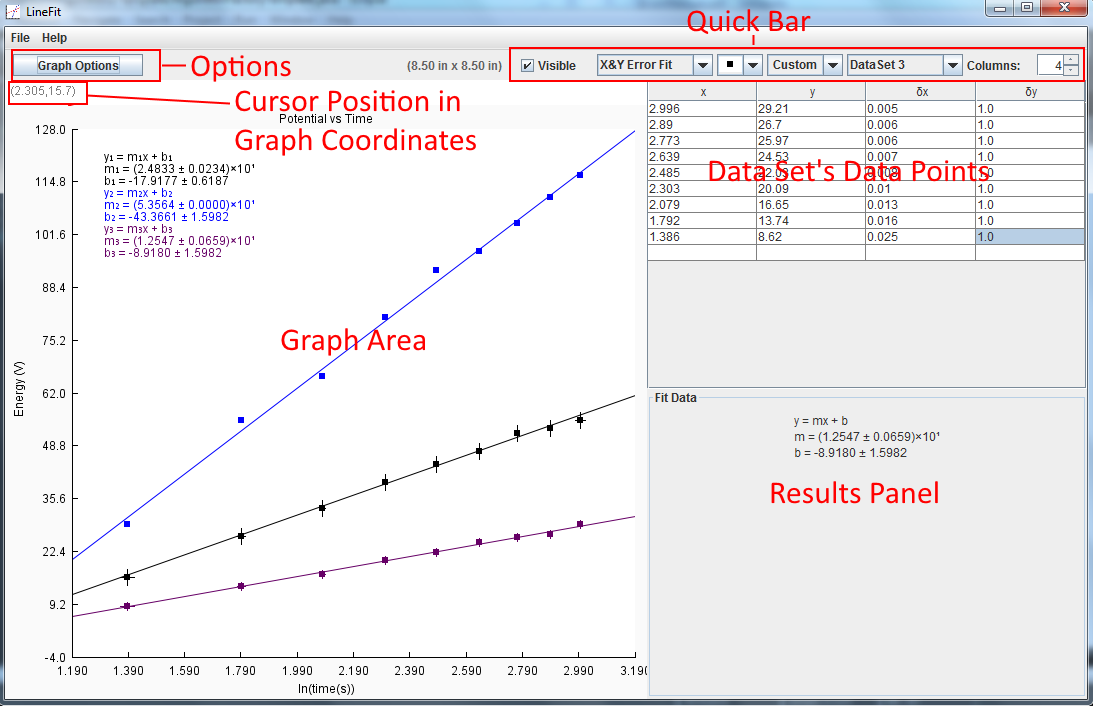
\includegraphics[width=15cm]{images/mainLineFitImage.png}
\caption{The main view of a LineFit Graph}
\end{figure}

\begin{itemize}
\item \textbf{Graph Area} - The main area where the graph and the data points are drawn.
\item \textbf{Data Set Data Points} - The table where the individual data points in a data set can be added/changed/removed.
\item \hyperref[sec:quickbar]{\textbf{Quick Bar}} - The area that houses many of the currently selected data set's options for displaying it in the graph area.
\item \textbf{Options} - The button that brings up the \hyperref[sec:options]{graph options menu} where many aspects of the graph can be changed.
\item \textbf{Results Panel} - The panel that contains the fit results for the currently selected data set.
\item \textbf{Cursor Position} - The position of the cursor on the application in the graph area's coordinates
\end{itemize}



\subsection{Quick Bar}
\label{sec:quickbar}

The quick bar is at the top of LineFit just below the menu bar. This bar houses many commonly used options for the data sets and also controls which data set is populated in the data points table.

\begin{figure}[ht!]
\centering
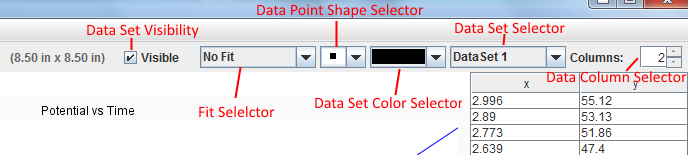
\includegraphics[width=15cm]{images/quickBar.png}
\caption{Close Up of the Quick Bar of LineFit Graph}
\end{figure}

\begin{itemize}
\item \textbf{Data Set Selector}- Drop down box that allows you to switch which data set's data is displayed in the quick bar, data points and results panel. New data sets can also be added through this selector by selecting the "New DataSet" option.
\item \textbf{Data Set Visibility Check Box} - Toggles whether or not the currently selected data set is visible in the graph area.
\item \textbf{Fit Selector} - Specifies which type of fit to use for this data set or if no fit should be used. This list is updated dynamically as data is entered into the data points table for this data set and check to see what, if any, error/uncertainty values are inputted. The possible fits, when the respective error/uncertainty values are present, are: No Fit, Regular Fit (no error/uncertainties), X Error Fit, Y Error Fit, and X\&Y Error Fit.
\item \textbf{Data Point Shape Selector} - Changes the shape to be displayed in the graph area for the data points in the currently selected data set. The current options are: Square, Circle, and Triangle.
\item \textbf{Data Set Color Selector} - Changes the color of the points, line, and results of the currently selected data set in the graph area. There is also the ability to choose any color by selecting the "Custom" option in the drop down which will pop up an interface that allows the user to select any color. There can only be one of these interfaces per data set so if you try and open it again, it will bring the already existing one to the front. The current options are: Black, Yellow, Blue, Green, Orange, Red, and Custom.
\item \textbf{Data Columns Selector} - A number spinner between 2 and 4 that is used to add or remove columns from the currently selected data set. The order the columns appear is: x, y, $\delta$y, then $\delta$x. If all four columns are being displayed, then $\delta$x is displayed before $\delta$y. If only errors in the x coordinates are desired then you must select the "use x errors" check box in the \hyperref[sec:options]{graph options menu}.
\end{itemize}



\subsection{File Menu}

This menu is displayed when the user selects the File button from the menu bar and allows for saving, exporting and loading files into or from LineFit.

\begin{figure}[ht!]
\centering
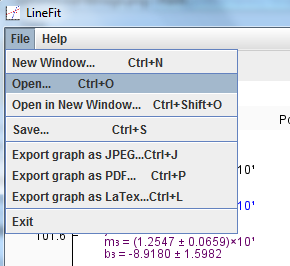
\includegraphics[width=7cm]{images/FileMenu.png}
\caption{The File Drop Down Menu}
\end{figure}

\begin{itemize}
\item \textbf{New Window} - Opens a new blank instance of LineFit. Key shortcut: Ctrl + N
\item \textbf{Open} - Opens the LineFit file (selected in the dialog that pops up) into the current instance of LineFit, putting the data sets read after any existing data sets. Key shortcut: Ctrl + O
\item \textbf{Open in New Window} - Opens the LineFit file (selected in the dialog that pops up) in a new instance of LineFit, not the current one. Key shortcut: Ctrl + Shift + O
\item \textbf{Save} - Opens a dialog that allows you to name and save the LineFit graph and options into a .txt file to be opened later by LineFit. Key shortcut: Ctrl + S
\item \hyperref[sec:exportjpg]{\textbf{Export graph as JPG}} - Opens a dialog that allows you to name and export only the content displayed in the graph area as a JPG image file. Note: This is not WYSIWYG so you should check to make sure it exports in a suitable fashion. Key shortcut: Ctrl + J
\item \hyperref[sec:exportpdf]{\textbf{Export graph as PDF}} - Opens a dialog that allows you to name and export only the content displayed in the graph area as a PDF file. Note: This is not WYSIWYG so you should check to make sure it exports in a suitable fashion. Key shortcut: Ctrl + P
\item \hyperref[sec:exportlatex]{\textbf{Export graph as LaTex}} - Opens a dialog that allows you to name and export only the content displayed in the graph area as a LaTex LineFit graph file. In order to use this in LineFit, you will need the linefit.sty file. Note: This is not WYSIWYG so you should check to make sure it exports in a suitable fashion. Key shortcut: Ctrl + L
\item \textbf{Exit} - Closes this instance of LineFit after prompting the user to save if there are unsaved changes.
\end{itemize}



\subsection{Help Menu}

This menu is displayed when the user clicks on the help button on the menu bar and provides some information and resources for LineFit.

\begin{figure}[ht!]
\centering
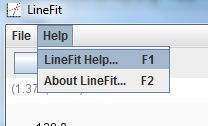
\includegraphics[width=5cm]{images/HelpMenu.png}
\caption{The Help Drop Down Menu}
\end{figure}

\begin{itemize}
\item \textbf{LineFit Help} - Opens up this PDF help document...
\item \textbf{About LineFit} - Opens up a small dialog that highlights some aspects of LineFit
\end{itemize}



\section{LineFit Options/Settings}
\label{sec:options}

This section explains each of the components on the options menu of LineFit and what they do. For convenience, it is broken up into four sections, \hyperref[subsec:axes]{Axes}, \hyperref[subsec:results]{Results}, \hyperref[subsec:export]{Export}, and \hyperref[subsec:dataset]{DataSet} options, based on the functionality the fields provide and have an effect on.

The options panel is responsible for making any change to the graphing area or to LineFit that is not accessible through the \hyperref[sec:quickbar]{quick bar}. These changes include things like changing the graph's name and the axes minimum and maximums. It should also be noted that multiple options menus can be opened at the same time allowing the user to switch between two sets of settings easily if they so desire.

\begin{figure}[ht!]
\centering
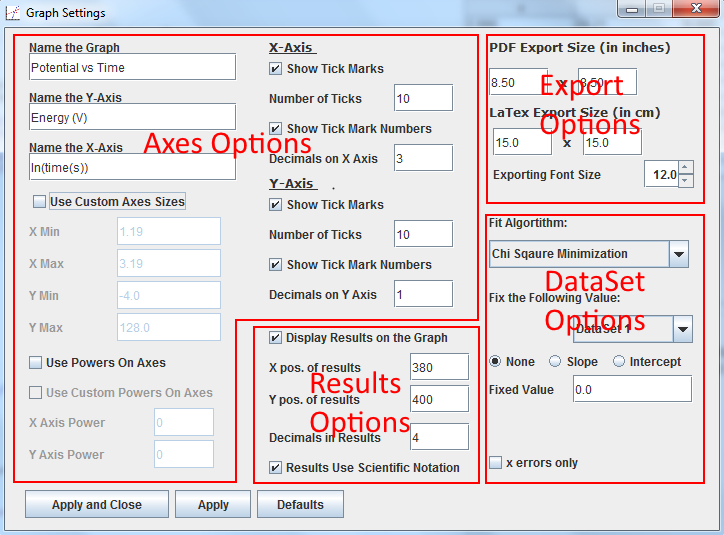
\includegraphics[width=15cm]{images/lineFitOptions.png}
\caption{The options/settings panel of LineFit}
\end{figure}

\begin{itemize}
\item \textbf{Apply and Close Button} - Applies any changes that have been made in the graph options menu to LineFit and then closes the menu.
\item \textbf{Apply Button} - Applies any changes that have been made in the graph options but does not close the window.
\item \textbf{Defaults Button} - Repopulates the values in the graph options to their default values but does NOT apply the changes. The user must hit either Apply or Apply and Close in order for the default settings to be applied.
\end{itemize}



\subsection{Axes}
\label{subsec:axes}

\begin{itemize}
\item \textbf{Name of the Graph} - The name of the Graph displayed above the graph in the main frame of LineFit. This is also the default name of any file created when saving or exporting. This name should be descriptive of what the graph shows a relationship between. Note: Unicode is supported and if the graph is being exported to LaTex, you can put LaTex formatted equations, such as \$(\textbackslash{}delta m)\^{}2\$, and they will display correctly in the PDF generated by LaTex.
\item \textbf{Name the Y-Axis} - The name of the y axis of this graph that is displayed to the left of the graph in the graph area. This name should be descriptive of what data is being used for the y (independent) values of the data sets. Note: Unicode is supported and if the graph is being exported to LaTex, you can put LaTex formatted equations, such as \$(\textbackslash{}delta m)\^{}2\$, and they will display correctly in the PDF generated by LaTex.
\item \textbf{Name the X-Axis} - The name of the x axis of this graph that is displayed to the below the graph in the graph area. This name should be descriptive of what data is being used for the x (dependent) values of the data sets. Note: Unicode is supported and if the graph is being exported to LaTex, you can put LaTex formatted equations, such as \$(\textbackslash{}delta m)\^{}2\$, and they will display correctly in the PDF generated by LaTex.
\item \textbf{Use Custom Axes Sizes} - If unchecked, which is the default, LineFit will adjust the axes automatically based on the visible data sets to put the points centered on the graph. If this box is Checked LineFit will NOT automatically adjust the minimum and maximum values and let the user specify them as well. By checking this, the X Min, X Max, Y Min and Y Max fields will become editable.
\item \textbf{X Min} - The user specified minimum value to use on the x axis. This will only be accessible if the Use Custom Axes Sizes check box is checked.
\item \textbf{X Max} - The user specified maximum value to use on the x axis. This will only be accessible if the Use Custom Axes Sizes check box is checked.
\item \textbf{Y Min} - The user specified minimum value to use on the y axis. This will only be accessible if the Use Custom Axes Sizes check box is checked.
\item \textbf{Y Max} - The user specified maximum value to use on the y axis. This will only be accessible if the Use Custom Axes Sizes check box is checked.
\item \textbf{Use Powers On Axes} - If checked, which is the default, powers of ten can be pulled out of the values along the axes and placed at the end of the axes to represent a quasi-scientific notation on the axes. If unchecked, the values are displayed on the axes without any powers of ten removed from them. This can help to shrink the size of the axes tick mark labels if they are too long and are overlapping each other.
\item \textbf{Use Custom Powers On Axes} - If unchecked, which is default, LineFit will determine the power of ten to extract from each of the axes so that the maximum value on each of them only has one digit in front of the decimal place. If checked, the user will then specify what powers of ten to use on each axis in the fields below. These two fields, X Axis Power and Y Axis Power, will only be editable if this check box is selected. This field will only be accessible if Use Powers On Axes check box is checked.
\item \textbf{X Axis Power} - The user specified power of ten to extract from each of the values on the X Axis to be displayed at the end of the axis. This will only become assessable if both the Use Powers On Axes check box and the Use Custom Powers On Axes check box are checked.
\item \textbf{Y Axis Power} - The user specified power of ten to extract from each of the values on the Y Axis to be displayed at the end of the axis. This will only become assessable if both the Use Powers On Axes check box and the Use Custom Powers On Axes check box are checked.
\item \textbf{X and Y Axes Tick Marks and Labels} - These options apply specifically to the marks and the number labels for each axis individually. These options are both available for each axis individually and are found below the respective axis header.

\begin{itemize}
\item \textbf{Show Tick Marks} - If checked, which is the default, tick marks will be drawn on the respective axis. If unchecked, not ticks or number labels will be drawn, only the axis line. The other mark and label options below this will be disabled for the respective axes if this is not checked.
\item \textbf{Number of Ticks} - The number of tick marks to draw on the respective axis line. This is only accessible if the Show Tick Marks check box for the respective axis is checked.
\item \textbf{Show Tick Mark Numbers} - If checked, which is default, the numbers that correspond with the tick locations will be drawn on the outside of the area formed by the axes for each tick mark. This is only accessible if the Show Tick Marks check box is checked. If this is unchecked, then the Decimals on \_ Axis will be disabled for the respective axis.
\item \textbf{Decimals on \_ Axis} - The number of decimal places to display for each of the number values on the respective axis. If this number is negative then it will round the results to that number of digits to the left of the decimal place. This is only accessible if the Show Tick Marks and Show Tick Mark Numbers check boxes for the respective axis is checked.
\end{itemize}

\end{itemize}



\subsection{Results}
\label{subsec:results}

\begin{itemize}
\item \textbf{Display Results on the Graph} - If this is checked, which is default, then the results of each data set that is visible will be displayed on the graph at the lower specified location relative to the bottom right corner of the graph area. If this is unchecked then the results will only be displayed in the results panel and the position options will be disabled.
\item \textbf{X pos. of results} - The x pixel offset of the leftmost result string to the right side of the graph relative to the bottom right corner of the graph area at which the results. This is the pixel distance between the right side of the graph and the end of the longest results string being displayed on the graph. It is important to remember that this is relative to the bottom right side of the graph area so it may move unexpected ways if you resize the LineFit window. Also, this is the part that will most likely be off when exporting to another file type for display outside of LineFit, but if it is exported as a \hyperref[sec:exlatexspace]{LaTex LineFit graph than this can be changed Later}. This will only be accessible if the Display Results on the Graph check box is checked.
\item \textbf{Y pos. of results} - the y pixel offset from the bottom of the lowest result string and the y axis of the graph. It is important to remember that this is relative to the bottom right side of the graph area so it may move unexpected ways if you resize the LineFit window. Also, this is the part that will most likely be off when exporting to another file type for display outside of LineFit, but if it is exported as a \hyperref[sec:exlatexspace]{LaTex LineFit graph than this can be changed Later}. This will only be accessible if the Display Results on the Graph check box is checked.
\item \textbf{Decimals in Results} - The number of decimal places to display in the results when drawing them on the graph or on the fit results panel. If this number is negative then it will round the results to that number of digits to the left of the decimal place.
\item \textbf{Results Use Scientific Notation} - If this is checked, which is the default, then the results will use scientific notation when being displayed and the suitable power of ten will be used so that the slope and intercept value will have only one digit in front of the decimal place. If unchecked then the number will be displayed in standard form with no power of ten taken out of it.
\end{itemize}



\subsection{Export}
\label{subsec:export}

\begin{itemize}
\item \textbf{PDF Export Size} - This allows the user to specify how big of a PDF image will be created when the graph is exported to a PDF file. The numbers in the two boxes below this label represent the width and the height (respectively) in inches of the PDF image created.
\item \textbf{LaTex Export Size} - This allows the user to specify how big of a LaTex LineFit graph will be created when the graph is exported to a LaTex file. The numbers in the two boxes below this label represent the width and the height (respectively) in centimeters of the LaTex graph created. This can be \hyperref[sec:exlatexspace]{changed later in the LaTex LineFit graph file} if desired.
\item \textbf{Export Font Size} - The font size that will be used when exporting the graph to any type of file. This allows the user to make the axes font (and the rest of the font too) smaller or larger if desired so that the graph can be readable. The spacing of the graph on on the axes is dependent on this so that the font will not overlap the graph regardless of the size. Once again, the\hyperref[sec:exlatexspace]{ LaTex LineFit graph font size can be changed later} if desired, but the spacing will not be updated automatically and will need to be done manually.
\end{itemize}



\subsection{DataSet}
\label{subsec:dataset}

\begin{itemize}
\item \textbf{Fit Algorithm} - The \hyperref[sec:algorithms]{linear fit algorithm} used when fitting lines to the data points in the data sets. This can be changed anytime, but the same fit is used for all of the data sets. The drop down box below this label allows the user to select the specific algorithm they want to use for this graph.
\item \textbf{Fix The Following Value} - The drop down below this label allows the user to choose a data set to edit what variable is fixed and the value for the fixed variable. The set of three radio buttons and the Fixed Value field is then populated with the selected data set's current values for these fields. These fields below the data set selector will be grayed out if the fit does not support fixing those variables or if the data set currently does not have a line fitted to it. The radio buttons then allow you to select whether no variable is fixed, in which case the Fixed Value is disables, or if the slope or intercept should be fixed.
\item \textbf{Fixed Value} - This is the value of the currently fixed variable chosen with the set of three radio buttons. This will be disable if "None" is selected or if the Fit Algorithm that is currently being used does not support fixing the variables.
\item \textbf{x errors only} - If unchecked, which is the default, then the third column (if there are only three columns in a given data set) in the data sets will be the y error/uncertainty value. If checked, the third column will instead be for the x error/uncertainty values for the data sets. This applies to all the data sets and not just the currently selected one. Also, if there are errors/uncertainties for both the x and y values than this does not have any effect and the x errors/uncertainties will always be displayed before the y ones.
\end{itemize}



\section{Saving and Exporting Graphs}



\subsection{LineFit File Format}

LineFit has its own file structure it uses when saving a LineFit file to be read back into LineFit later. While it does represent a unique structure, it has been intentionally left as a .txt file extension. This is so that users will realize that it is a human readable file and is designed so that the contents are easy to see and understand. What the key words store the value for should be obvious and each graph option has its own line in the file. Note that not all the lines need to be there and if any option is removed it will use the default value for that option.

\begin{figure}[ht!]
\centering
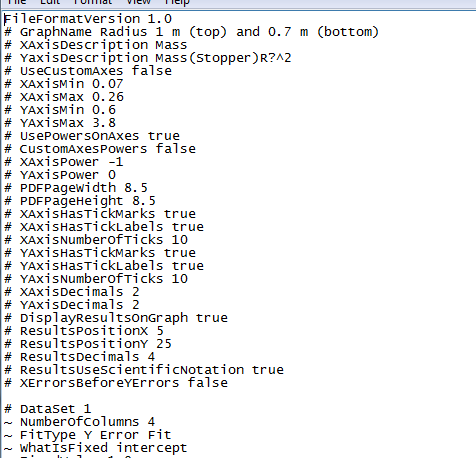
\includegraphics[width=7cm]{images/saveFile.png}
\caption{An example LineFit .txt save file}
\end{figure}

The file consists of many lines starting with one of two "keys" follows by a keyword name and then the value that goes with the keyword name. The first key is the "\#" sign which means that the line is a graph option that has been saved to the file. This is true for all but when the line is "\# dataset ...", which means that the file will now read in the data set values until it reaches an empty line. The "\~{}" is the key that denotes that the line is data for the data set that is currently being read in. Also, the order of these lines is, for the most part, arbitrary. The only thing that matters is that after the "\#dataset ..." the next lines until an empty line contain all the information for that data set denoted with the "\~{}."



\subsection{Exporting the Graph}

LineFit also currently supports three ways to export your graph so that it can be seen and used outside of LineFit. The three options for exports are as a JPG image, a PDF image, or as a LaTex LineFit graph file. It is important to note that none of these exports are what you see is what you get (WYSIWYG), meaning that the proportions of the exports will not necessarily be the same as they are in LineFit. The graph itself will not change, but the text and spacing of the graph may be different and the most notably and often different part is where the results of the fits are displayed on the graph. Because of this, it is always important that you check the export files to make sure they are suitable and then re-export them if the are not using different settings in the graph options menu. None of these export files can be read back into LineFit so it is always recommended that you save your file as a LineFit .txt file as well in case you need to change something about the graph later since the two image exports are completely static and the LaTex graph file is not easily changed.



\subsubsection{JPG and PDF Image Exports}
\label{sec:exportjpg}
\label{sec:exportpdf}

The first two export options are standard image files and can be used as such. The images created with these exports are completely static and cannot be changed after they are exported. If they do not export how you would like them to then you must change the options in LineFit and export it again. Because of this, it is very important to either save your LineFit file as a .txt file or to make sure your export image is suitable and no text overlaps in them. Once again, this is not a WYSIWYG export so it will not match proportionally exactly what is displayed in LineFit and should also be save as a LineFit .txt file since the exports cannot be read into LineFit.



\subsubsection{LaTex LineFit Graph Export}
\label{sec:exportlatex}

The LaTex LineFit graph export option is designed only for use in LaTex documents and requires the linefit.sty file in order to draw the graph which can be found at the same place as the LineFit.jar file on the LineFit page hosted on Covenant College Physics website under the student resources section. This export is designed to be copied over to a LaTex file where it will dynamically draw the graph using the linefit.sty file. Because it is dynamically drawn, spacing and other aspects of this export graph can be changed, although not as easily as changing them in LaTex. How to do this is described \hyperref[sec:exlatexspac]{below}. Once again, this is also not a WYSIWYG export so it will not match proportionally exactly what is displayed in LineFit and should also be save as a LineFit .txt file since the exports cannot be read into LineFit.



\subsubsection{Changing Aspects of the LaTex LineFit Graph Export}
\label{sec:exlatexspace}

To explain how the spacing works in the LaTex LineFit graphs, it would be easiest to walk through a sample file and explain each line of code and the spacing options on it. The graph is broken up into three main sections separated by new lines. The first three lines set up the graph area. The next set of lines represents a data set and there will be one of these sections for each data set in the LaTex graph. The final section draws the axis of the LaTex graph.

\begin{figure}[ht!]
\centering
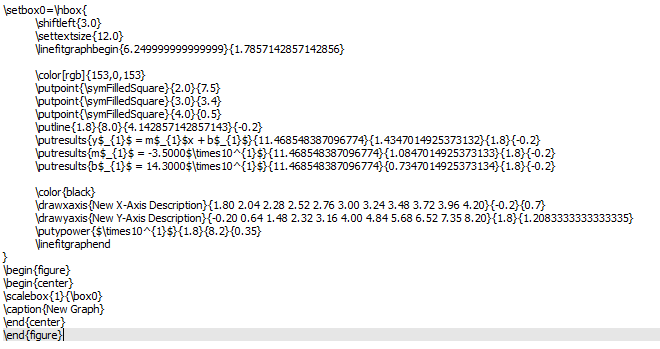
\includegraphics[width=14cm]{images/latexFile.png}
\caption{An example LaTex LineFit graph file}
\end{figure}

\textbf{First Section - Setting up the Graph}
\begin{itemize}
\item \textbackslash{}shiftleft\{number\} - This command shifts the entire LaTex graph to the left by the specified number of centimeters. If you graph is off the end of the page, consider changing this shift to be larger.
\item \textbackslash{}settextsize\{number\} - This command sets the font size in LaTex to the given point size. Note that the spacing on the axes will NOT change automatically based on this.
\item \textbackslash{}linefitgraphbegin\{number\}\{number\} - This tells LaTex that we are beginning to draw the graph and sets up the correlation between centimeters and units on the graph. The two numbers are the x and y units to pixel ratios and this should almost never be changed.
\end{itemize}

\textbf{Second Section - Drawing Data Sets}
\begin{itemize}
\item \textbackslash{}color[rgb]\{red, green, blue\} - This sets the color that anything after it will be drawn to the graph with using the inputted 0-255 rgb values. The [rgb] specifies that it uses this format for the color. If you use a predefined color it will be in the format of \textbackslash{}color\{predefinedColor\}
\item \textbackslash{}putpoint\{\}\{\}\{\} - This places the points on the graph and should not be changed
\item \textbackslash{}putline\{\}\{\}\{\}\{\} - This draws the line through the points on the graphs and should not be changed
\item \textbackslash{}putresults\{string\}\{xCmToDrawAt\}\{yCmToDrawAt\}\{\}\{\} - This places the given string of text on the graph at the passed x and y values on the graph (not in cm). If the results locations are not correct or overlap, change the values of where the results are drawn at.
\end{itemize}

\textbf{Third Section - Drawing the Axes}
\begin{itemize}
\item \textbackslash{}draw\_axis\{\}\{\}\{\}\{labelSpacing\} - This draws the respective axis of the graph with the given label at the spacing number of cm below or to the left of the axis line. This is the only value that should be changed.
\item \textbackslash{}draw\_axisforsmallvalues\{\}\{\}\{\}\{\}\{labelSpacing\} - Same as the other draw axis command, but this is used when small values are being graphed so that they are still drawn correctly.
\item \textbackslash{}put\_power\{powerString\}\{\}\{\}\{spacing\} - Draws the power string for the respective axis spaced the given amount in cm from the end of the axis.
\item \textbackslash{}linefitgraphend - This tells LaTex that we are done drawing the graph
\end{itemize}



\section{Linear Fit Algorithms}
\label{sec:algorithms}

This section will describe how to manipulate data so that it can be fit using a Line. In addition, each of the different Fit Algorithms that are available in the current version of LineFit will be described. Each sub section will explain and demonstrate how the algorithm fits data, why this approach is useful/practical, and the benefits and disadvantages of each algorithm. Each sub section will also explain how the algorithm is modified to allow for fixing the slope or intercept if they allow this.



\subsection{Data Manipulation to be Fit With Lines}
\label{sec:dataManipulation}

Comming soon...

\subsection{Quadratic Minimization}

Comming soon...

\subsection{Partial Derivative Minimization}

Comming soon...

\end{document}
